% !TeX root = ../main.tex
\section{Homology} % (fold)
\label{sec:homology}

% Simplicial complexes not only provide a comprehensive discretization of continuous domains, but are the primary tool for concrete calculations in algebratic topology.
% In particular, the study of simplicial homology groups and its dual cohomology groups rely on simplicial complexes in order to study important topological invariants of a discretized space.
%
% \subsection{Homology}

The following vector spaces may be defined over any field $\F$, however we will assume the field $\F_2$ in order to avoid orienting the simplices in $K$.
Let $C_k(K)$ denote the vector space over some field $\F$ consisting of linear combinations of $k$-simplices in $K$, which form a basis for $C_k(K)$, known as \textbf{$k$-chains}.
These vector spaces are connected by \textbf{boundary maps} $\partial_k:C_k(K)\to C_{k-1}(K)$ which are linear transformations taking basis elements of $C_k(K)$ to the abstract sum of basis $(k-1)$-simplex faces.
The collection of chains and boundary maps forms a sequence of vector spaces known as the \textbf{chain complex} $\C = (C_*,\partial_*)$
\[
    \ldots\xrightarrow{\partial_{k+1}}
    C_k(K)\xrightarrow{\partial_{k}}
    C_{k-1}(K)\xrightarrow{\partial_{k-1}}
    \ldots\xrightarrow{\partial_2}
    C_1(K)\xrightarrow{\partial_{1}}
    C_0(K)\xrightarrow{\partial_0} 0.
\]

An important property of the boundary maps $\partial_k$ is that the composition of subsequent boundary maps is zero.
That is, for all $k$
\[
  \partial_k\circ\partial_{k-1} = 0.
\]
As a result the image of $\partial_{k+1}$, denoted $\im\partial_{k+1} = \{\partial_{k+1}c\mid c\in C_{k+1}(K)$ is a subspace of the kernel, $\ker\partial_k = \{c\in C_k(K)\mid \partial_k c = 0\}$, of $\partial_k$.
A \textbf{$k$-cycle} of $\C$ is a $k$-chain with empty boundary---an element of $\ker\partial_k$.
Two cycles in $\ker\partial_k$ are said to be \textbf{homologous} if they differ by an element of $\im\partial_{k+1}$.
This leads us to the definition of the \textbf{homology groups} of $K$ as quotient vector spaces $H_k(K)$ over $\F$, defined for $k\in\N$ as
\[
  H_k(K) := \ker\partial_k/\im\partial_{k+1}.
\]

The rank of a homology group is of particular importance and is known as the \textbf{Betti number} $\beta_k = \rank H_k(K)$.
These topological invariants can be thought of as counting the number of $k$-dimensional ``holes'' in a topological space, where $0$-dimensional holes are connected components, $1$-dimensional holes are loops, $2$-dimensional holes are voids, and so on.
Note that this is the same notion which motivated our use of simplicial complexes for determining coverage---a $1$-dimensional hole exists if a gap in a neighborhood graph cannot be filled by triangles.

\subsection{Relative Homology}

\begin{figure}[htbp]
\centering
    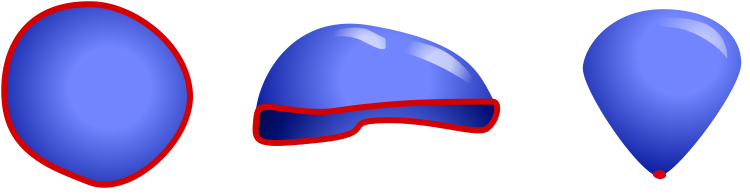
\includegraphics[scale=0.5]{figures/balloons1.png}\vspace{2ex}
    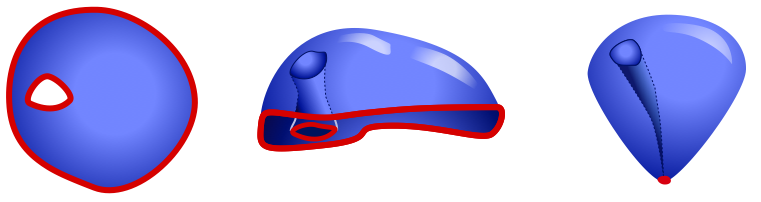
\includegraphics[scale=0.5]{figures/balloons3.png}
    \caption{(Left) Two connected, planar domains with boundaries (in red).
            We can gather some intuition for the relative homology of a pair $(\D,\B)$ by thinking about wrapping the interior of the domain around its boundary, and identifying all points in the boundary with a point (Right).
            Even with disconnected boundaries we know that $\beta_2 = \rank~ H_2(\D, \B) = 1$.  That is, there is just one enclosed void.}
    \label{fig:balloons1}
\end{figure}

For a simplicial complex $K$ let $L\subset K$ be a subcomplex of $K$.
Let $\C(K, L)$ denote the quotient chain complex of pairs $(C_k(K, L), \overline{\partial_k})$ where $C_k(K, L) = C_k(K)/C_k(L)$ consists of the chains on $K$ modulo chains on $L$, with the induced boundary maps $\overline{\partial_k}$ on the quotients.
Each relative chain is an equivalence class of chains in $K$ which are identical without the elements of $L$.
The \textbf{relative homology groups} $H_k(K, L)$ consists of homology classes of relative cycles - chains in $K$ whose boundaries vanish or lie in $L$.
That is, a relative cycle can either be a cycle in $K$ or a chain in $K$ with a boundary in $L$.

As we will see, relative homology provides a powerful representation of a bounded domain that is particularily suited to verifying coverage of a sensor network.
Let $\D$ be a bounded domain with boundary $\B\subset\D$.
For illustrative purposes assume $\D$ is a connected, compact subset of the euclidean plane $\R^2$ so that certain properties of the relative homology of the pair $(\D, \B)$ are known.
Namely, there is exactly one equivalence class in $H_2(\D, \B)$, as illustrated in Fig.~\ref{fig:balloons1}.
We can think of the quotient as an identification of points in the boundary, illustrated by wrapping the planar domain around a single point in $\R^3$.
As the domain is compact this creates a single void corresponding to the one generator in $H_2(\D, \B)$.

\begin{figure}[htbp]
\centering
    
\includegraphics[scale=0.5]{figures/balloons2.png}
    \caption{If there is a gap in the domain that is not a part of the boundary then $\beta_2 = \rank~ H_2(\D, \B) = 0$ as there is no void.}
    \label{fig:balloons2}
\end{figure}

Now suppose our network $P$ covers the domain at some scale $\alpha > 0$ such that there are no gaps (1-cycles) in $\rips^\alpha(P)$.
The subset $Q = \{p\in P\mid \ball_\alpha(p)\cap\B\neq\emptyset\}$ of points within distance $\alpha$ of $\B$ induces a subcomplex $\rips^\alpha(Q)$ of $\rips^\alpha(K)$.
Under our assumptions, the relative homology $H_2(\rips^\alpha(K), \rips^\alpha(Q))$ should reflect that of the domain.
A gap in coverage can be thought of as ``popping the balloon'' in the sense that, if we wrap the simplices of $\rips^\alpha(K)$ around those in $\rips^\alpha(Q)$ we would have no void---the gap provides a hole through which the ``air'' can escape, as illustrated in Fig.~\ref{fig:balloons2}.

\subsection{Functions and Filtrations}

\begin{figure}[htbp]
\centering
    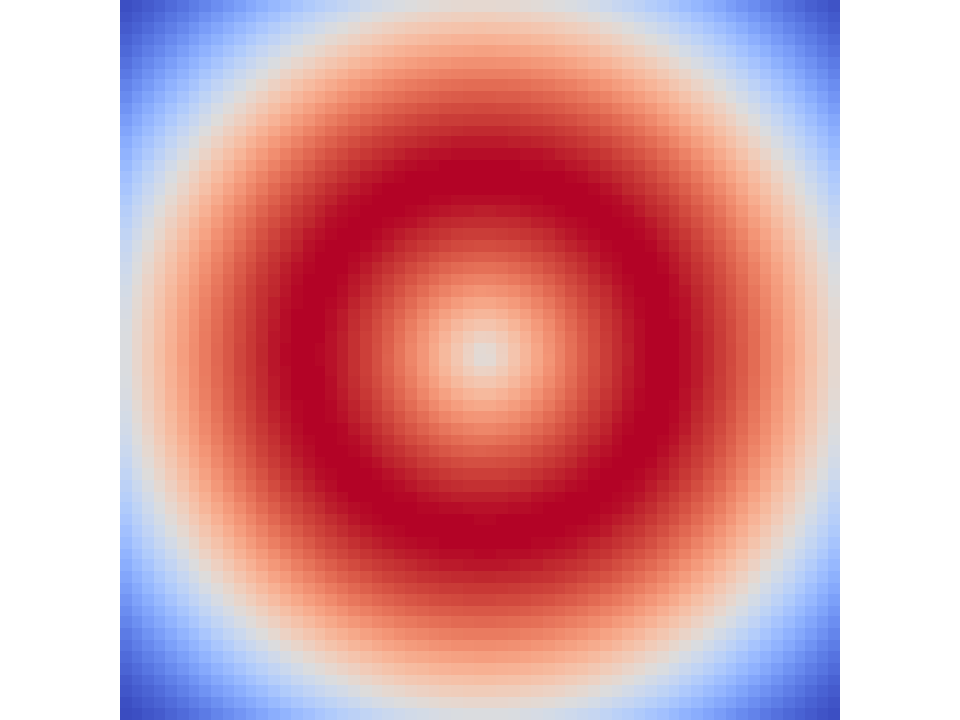
\includegraphics[scale=0.45]{figures/fgrid.pdf}
    % 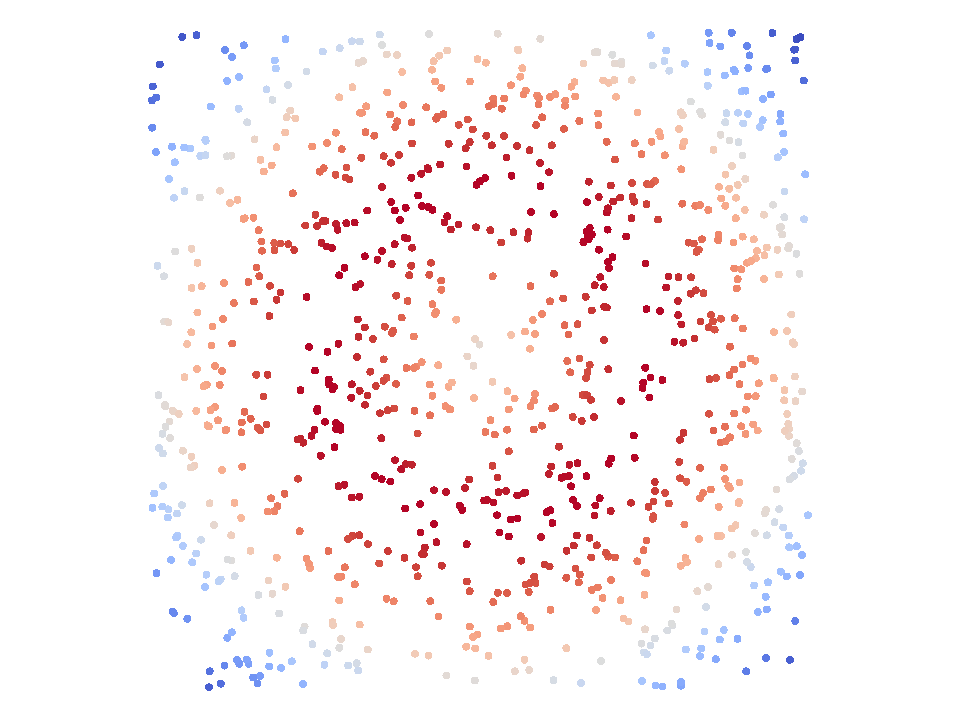
\includegraphics[scale=0.45]{figures/fsample.pdf}
    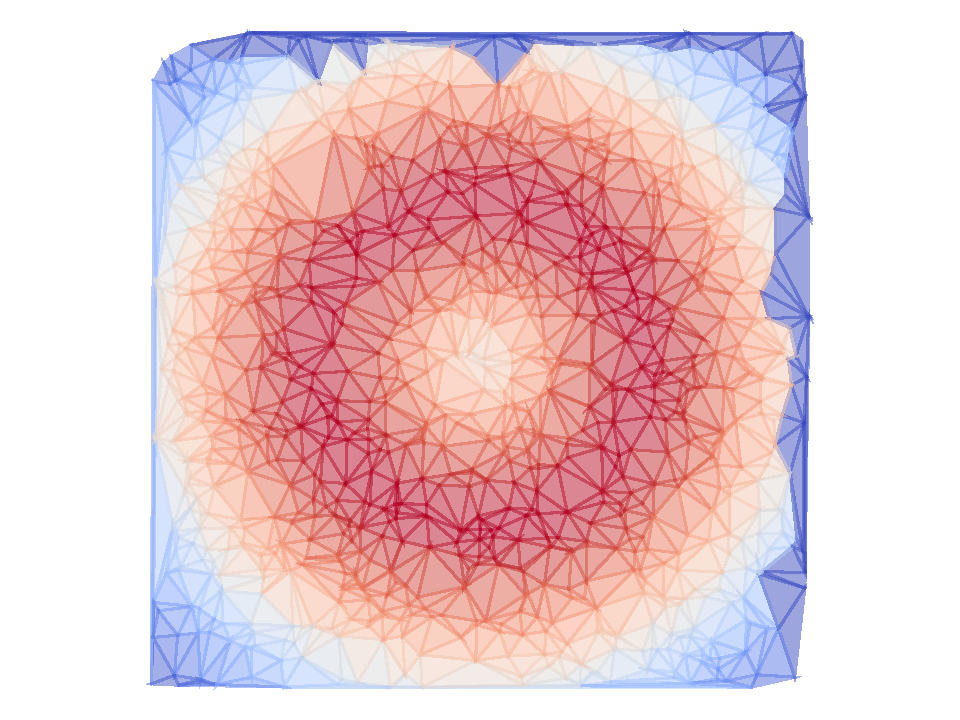
\includegraphics[scale=0.55]{figures/fcomplex.pdf}
    \caption{(Left) Continuous function on the plane.
            % (Middle) Function values on random sample.
            (Right) Function values on a random sample extended to a continuous piecewise linear approximation on a 2-dimension simplicial as the $z$-axis.}
    \label{fig:function}
\end{figure}

Suppose we have some real valued function $f:\D\to\R$ and endow our sensors with the ability to measure this function at their points $P$.
If we know our network covers the domain we may construct a simplicial complex which captures its topology in a discrete structure.
We may therefore integrate the sparse measurements provided by the sensors throughout the simplicial complex to capture the topology of the function itself.
Not only do we now have a discrete approximation of the function but an ordering on the simplices of the complex which may be used to explore the evolution of the topological structure of the function.

This leads to a more general notion defined for a sequence of topological spaces, which we may take as sublevel sets of the function on the domain.
\begin{definition}
    Let $f:\D\to\R$ be a function on a topological domain $\D$ and let $I_0, I_1,\ldots$ be a sequence of intervals $I_i = [a_i, b_i)$ that covers the image of $f$ on $\D$.
    Let and $X_i = \{x\in\D\mid a_i\leq f(x) < b_i\}$ be topological subspaces connected by inclusion maps $X_i\to X_{i+1}$.
    A \textbf{filtration} is the resulting sequence of topological spaces
    \[X_0\to X_1\to\ldots X_i\to X_{i+1}\to\ldots .\]
\end{definition}
A filtration $\{K_i\}_{i=1,\ldots,n}$ may also be interpreted as a sequence of simplicial maps, each an inclusion $K_i\to K_{i+1}$.
This induces an algebraic sequence of homomorphisms on homology by functoriality, for all $k$:
\[ H_k(X_0)\to H_k(X_1)\to\ldots\to H_k(X_i)\to H_k(X_{i+1})\to\ldots . \]
This sequence encodes the local topological changes that occur at each step of the filtration.
Global information is encoded in terms of the \textbf{birth} and \textbf{death} of homology classes, represented as a \textbf{persistence diagram} or \textbf{barcode}.

% \vspace{0.25in}
% \textbf{TODO} Persistence diagram of a function on a simplicial complex
% \vspace{0.25in}

\begin{figure}[htbp]
\centering
    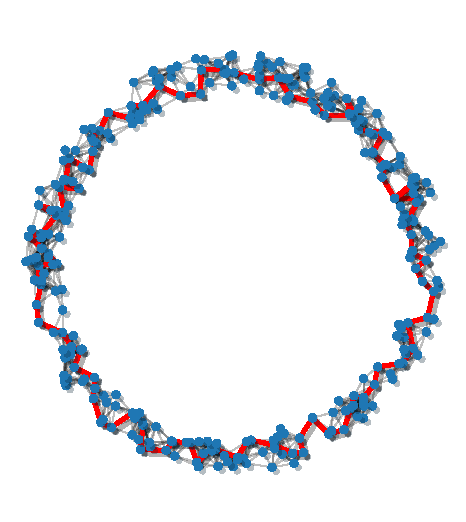
\includegraphics[scale=0.9]{figures/homology_cycle.pdf}\hspace{10ex}
    % 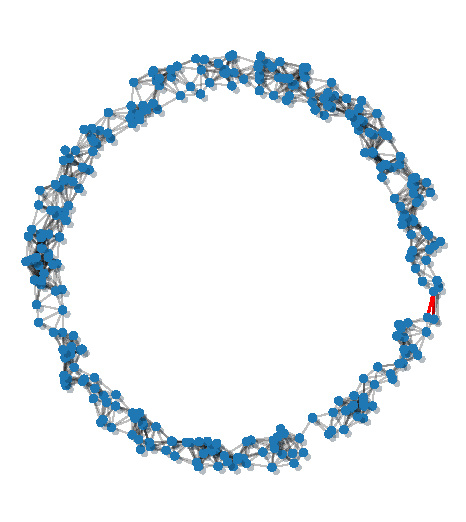
\includegraphics[scale=0.6]{figures/cohomology_cocycle.pdf}
    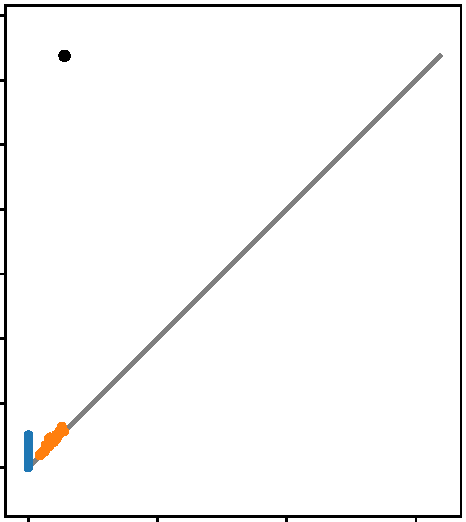
\includegraphics[scale=0.8]{figures/homology_dgm.pdf}
    \caption{The representative cycle of a significant feature in the persistent homology of rips filtration of a noisy circle.
            The birth of the feature indicated on the persistence diagram (right) corresponds to the scale of the rips complex shown (left) when the circle, a 1-cycle, is born.
            The death of this feature corresponds to the scale of the rips complex at a larger scale (not shown) when a triangle first fills the interior of the circle.
            This scale is approximately the length of the edges in the smallest equilateral triangle with sample points as vertices that contains the centroid of the sample.
            This illustrates the geometric information encoded in the persistence diagram of geometric complexes as it is within a constant factor of the radius of the circle.}
    \label{fig:cycle_diagrams}
\end{figure}

Given a simplicial complex $K$ on a set of points $P\subset\D$ and a function $f:\D\to\R$ we may construct a filtration $\{K_i\}_{i=1,2,\ldots}$ by ordering the simplices by their function values.
For example, $f(\sigma) = \max_{v\in\sigma} f(v)$ for any simplex $\sigma\in K$.
The resulting filtration is now a sequence of simplicial maps, each an inclusion $K_i\to K_{i+1}$, which induces a sequence of homology groups.

\subsection{Persistent Homology}

\begin{figure}[htbp]
\centering
    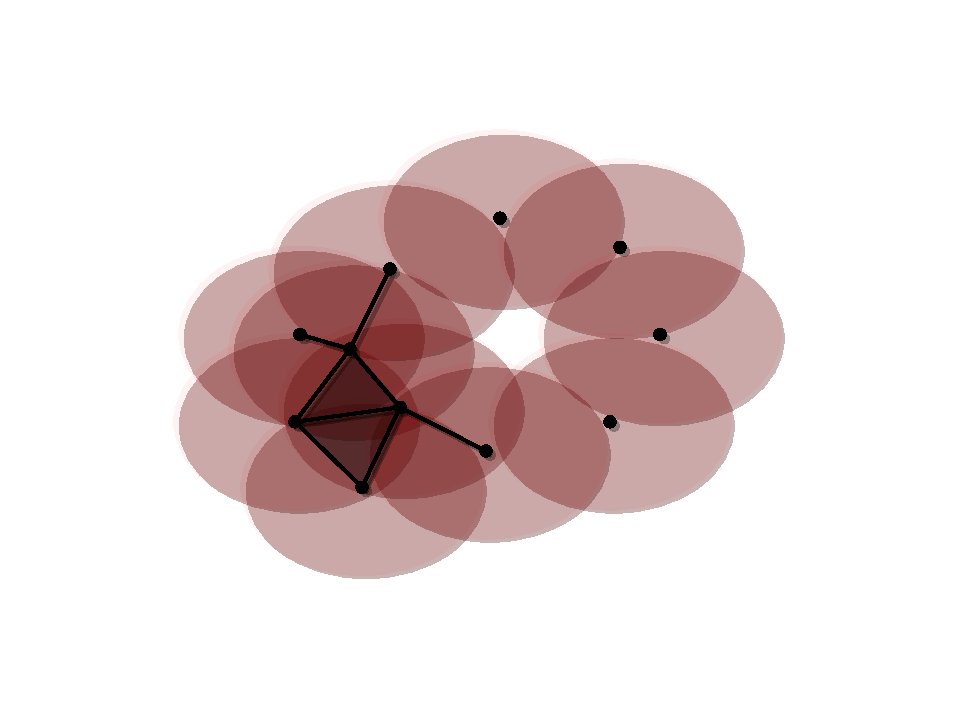
\includegraphics[scale=0.4]{figures/persist06.pdf}
    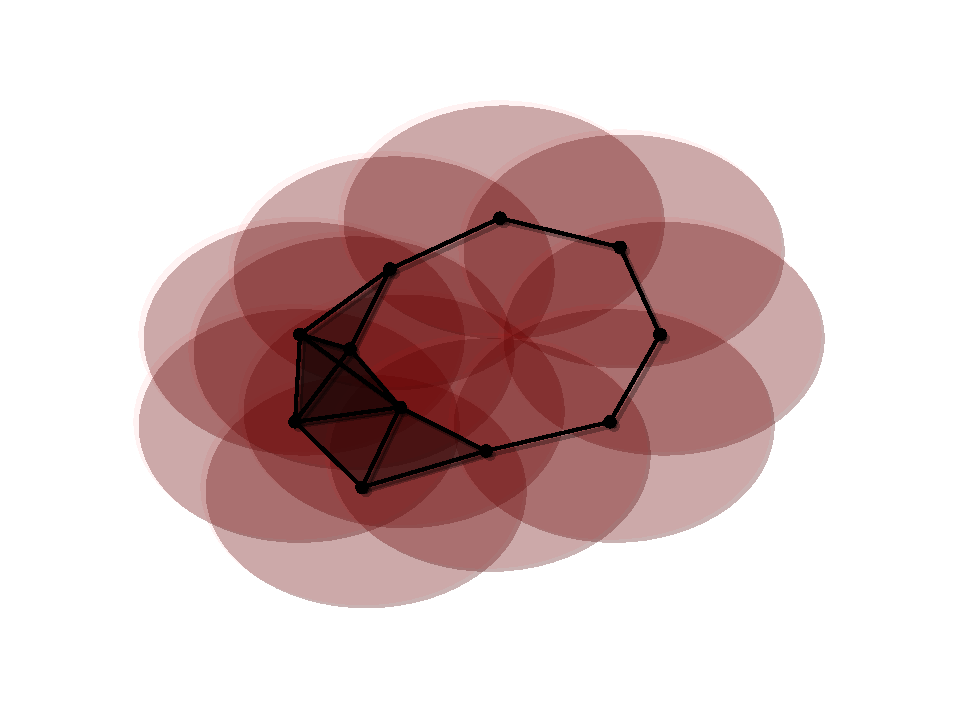
\includegraphics[scale=0.4]{figures/persist08.pdf}
    % 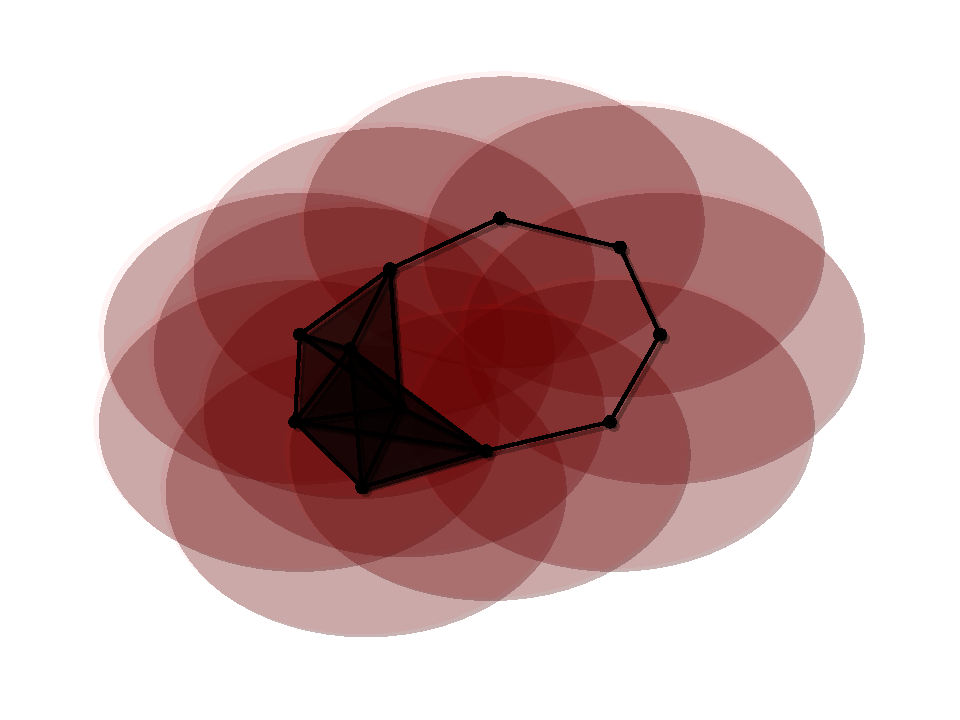
\includegraphics[scale=0.4]{figures/persist10.pdf}
    % 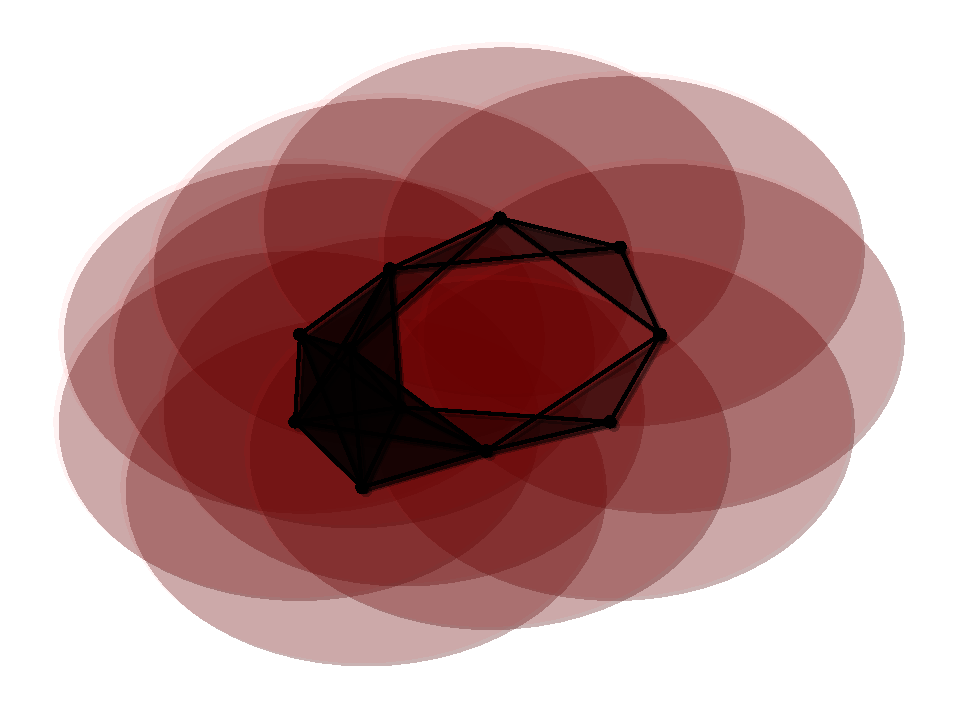
\includegraphics[scale=0.4]{figures/persist12.pdf}
    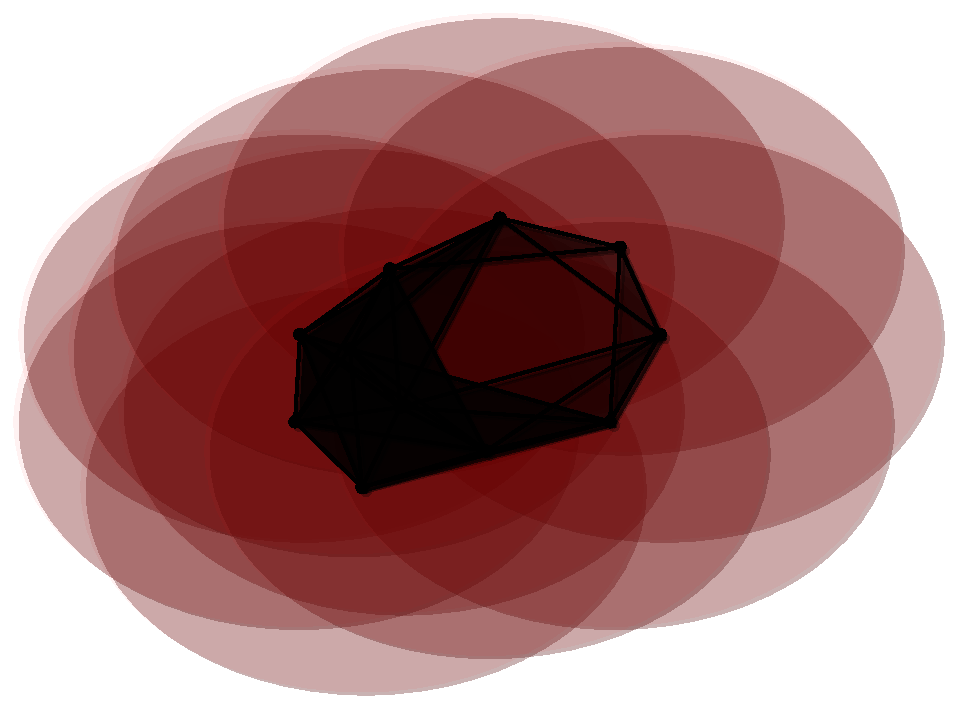
\includegraphics[scale=0.4]{figures/persist14.pdf}
    \caption{A filtration of rips complexes at scales 0.6, 0.8, and 1.4 illustrating a point $(0.8, 1.4)$ in the corresponding persistence diagram. The 1-cycle that is born at scale 0.8 persists until it dies at scale 1.4.}
    \label{fig:persist}
\end{figure}

% \vspace{0.25in}
% \textbf{TODO} ``Metric'' persistence.
% \vspace{0.25in}

% Topological data analysis is an emerging field in the intersection of data analysis and algebraic topology which extends the notion of homology and cohomology groups to a more analytical tool known as \textbf{topological persistence}.
% Where simplicial homology identifies invariants of a static simplicial complex persistent homology tracks the evolution of a sequence of nested simplicial complexes which provide a more detailed topological signature, in addition to relevant geometric information.

Just as we can construct a filtration from a function on a simplicial complex we can construct a filtration from the metric induced on our sample by the domain.
Let $P$ be a finite metric space with $m$ points and let $K = \rips^\alpha(P)$ be the Rips complex of $P$ at scale $\alpha$ consisting of $n$ simplices.
We can order the simplices $\sigma_1,\ldots,\sigma_n$ by the minimum pairwise distance between their vertices by first applying an arbitrary ordering on the vertices $v_1,\ldots,v_m$ and letting $\sigma_i = \{v_i\}$ for $i=1,\ldots,m$ so that $K_i = \{\sigma_1,\ldots, \sigma_m\}$.
We can then build a filtration $\K = \{K_i\}_{i=1,\ldots,n}$ so that $K_i = \rips^\e(P)$ where $\e = \max_{u,v\in\sigma_i}\dist(u,v)$ by adding one simplex at a time, breaking ties first by dimension, then by the ordering on their constituent vertices.
A $k$-dimensional feature is identified when a $(k+1)$-simplex $\sigma$ is added that kills a $k$-cycle $\gamma$.
In the persistence diagram, this feature would be represented by a point $(b, d)$ where $b$ is the smallest scale for which the $k$-cycle appears
\[ \tau\in\rips^b(P)\text{ for all }\tau\in\gamma\]
and $d = \max_{u,v\in\sigma}\dist(u,v)$ is the scale at which $\sigma$ enters the filtration.
The result is a collection of points $(b_i, d_i)$ in the plane for each dimension $k$ known as the persistence diagram, denoted $\dgm_k(\K)$.
A persistence diagram is depicted on the right in Fig.~\ref{fig:cycle_diagrams}.

% section homology (end)
